\documentclass[12pt,a4paper]{article}
%\renewcommand{\familydefault}{\ttdefault}
\pagenumbering{gobble} %remove page number
\usepackage[font=small,labelfont=bf]{caption} % Required for specifying captions to tables and figures
\usepackage{lmodern} %to fight font errors
\usepackage{array,booktabs,ragged2e}%centering tables 
\usepackage{polski}
\usepackage[utf8]{inputenc} 
\usepackage{blindtext}
\usepackage{longtable}
\usepackage[left=1.0cm,right=1.0cm,top=1cm,bottom=0.0cm]{geometry}
\usepackage{multirow}
\usepackage{verbatim}
\usepackage{multicol}
\setlength\columnsep{-6.0cm} % This is the default columnsep for all pages
\usepackage{tabularray}
\usepackage{graphicx}
\usepackage{hyperref}
\usepackage{indentfirst} % indent first paragraph
\usepackage{enumitem} %[leftmargin=*]

\hypersetup{colorlinks=true,linkcolor=blue,urlcolor=blue}

\usepackage{color}
\definecolor{techColor}{RGB}{120, 120, 120}

\begin{document}

\begin{tabular}  { >{\RaggedLeft} p{16cm}  p{3cm} }  
	{\Large \textbf{KRZYSZTOF BOBNIS}} \hfill Wrocław & \textcolor{techColor}{residence} \\
	 GAME PROGRAMMER, GAME JAMMER \hfill  {\href{mailto:kbobnis@gmail.com}{kbobnis@gmail.com}} & \textcolor{techColor}{email} \\ 
	 \hfill {\href{https://www.linkedin.com/in/krzysztofbobnis}{linkedin.com/in/krzysztofbobnis}} & \textcolor{techColor}{linkedin} \\
	 \hfill {\href{http://bobnis.eu}{bobnis.eu}} & \textcolor{techColor}{portfolio} \\
	 \hfill {\href{https://github.com/kbobnis}{https://github.com/kbobnis}} & \textcolor{techColor}{github} \\
\end{tabular}	 

\vspace{0.5cm}

\begin{multicols}{2}

\centering
\section*{Summary}
\justifying

	Graduated from Wrocław University of Technology with AI and advanced computer graphics specialties. My thesis was based on fractal structures and genetic algorithms. During that time we learned c++ and wrote several experimental programs in it. After that worked as a programmer for 11 years (8 years in game dev). I have created 23 games, most on game jams as prototypes, several of them polished and published.
	\\

	\textbf{Excellent with}: Unity3d, c\#, php, google play store, git, svn, communication, english, game design, UX.

	\textbf{Good with}: C++, java (native android), as3, app store, algebra, AI, computer graphics.

\centering
\section*{Experience }
\justifying
	 {\large \textbf{Tech Lead}}  \hfill \textcolor{techColor}{unity, c\#, CI integration, automated tests} \\
	{\href{https://dali.games/}{Dali Games}}  / \textit{Poland}, 2020 - present  \\
	Creating adventure creator tool called Dali Engine that is used in two games with 200,000+ downloads: {\href{https://play.google.com/store/apps/details?id=games.dali.adventure.neighborhood.unholy}{Unholy Neighbourhood}}, {\href{https://play.google.com/store/apps/details?id=games.dali.adventure.reborn}{Reborn Adventure}} \\

	{\large \textbf{Senior Programmer}} \hfill \textcolor{techColor}{unity, c\#, git, google fit, apple health} \\
	{\href{https://cat-astrophe-games.com/}{Cat-astrophe-games}}  / \textit{Poland}, 2020 \\
	Unreleased project. Created working prototype of run / walk / steps verifier as a game on a mobile phone   \\

	{\large \textbf{Programmer, later Senior Programmer}} \hfill \textcolor{techColor}{unity, AR, c\#, ruby, redis, mysql, video streaming} \\
	{\href{https://www.uken.com/}{Uken}}  / \textit{Canada}, 2017 - 2018 \\
	Developed {\href{https://play.google.com/store/apps/details?id=com.uken.pool}{Kings of Pool}} game for mobile with AR mode with \textgreater 500,000 downloads. Duties involved developing game in every aspect. Later unreleased project: duties involved working on video player streaming over internet and regular contact with 3rd party representatives. \\

	{\large \textbf{Programmer}} \hfill \textcolor{techColor}{unity, c\#, php, redis, git, as3} \\
	{\href{https://tensquaregames.com/}{TSG}}   / \textit{Poland}, 2012 - 2015, then 2016 - 2017 \\
	Developed {\href{https://play.google.com/store/apps/details?id=air.com.tensquaregames.letsfish}{Lets-Fish}} game for web in as3, later on mobile in unity with 10M+ downloads. Duties involved developing new features with strict collaboration with UI artists and game designers. \\

	{\large \textbf{Student}} \hfill \textcolor{techColor}{c\#, c++, java, as3} \\
	{\href{https://pwr.edu.pl/en/}{Wroclaw University of Technology}}  / \textit{Poland}, 2006 - 2011  \\
	Graduated, Master of Science in Information Technology. Major: Computer Science. Educational profiles: \textbf{Artificial Intelligence, Advanced Computer Graphics, Computer Networks}.



\begin{itemize}[leftmargin=7.0cm]
	\centering
	\section*{After hours}
	\justifying
	\setlength\itemsep{0.0cm}
	\item[]  \textbf{C++ / SFML / STL} / Created a tetris game {\href{https://github.com/kbobnis/tetris}{github link}}. \\
	\item[] \textbf{Co-created {\href{https://www.facebook.com/events/1110429105711126}{"Sensei" Game Jam 2016}}} / with 120 attendees in Wroclaw's University. \\
	\item[]  \textbf{Won Game Jam} / 1st place on TK Game Jam: {\href{https://itch.io/jam/tk-game-jam-2016/results}{itch.io}}. \\
	\item[] \textbf{Self publisher} / Published 4 games, one of them {\href{https://play.google.com/store/apps/details?id=com.wyspianStudios.rpgModuleFull}{RPG Module}} made US\$10,000+. \\
	\item[] \textbf{23 game prototypes} / Used Unity (Unreal was used once), all projects can be viewed on  {\href{http://bobnis.eu}{bobnis.eu}}. \\
\end{itemize}

\begin{itemize}[leftmargin=7.0cm]
	\centering	
	\section*{Languages}
	\justifying
	\setlength\itemsep{0.0cm}
	\item[] \textbf{English} - \textbf{fluent}: passed ACERT: C1 english certificate, lived for 3 years in Canada.
	\item[] \textbf{Polish} - \textbf{native}: born and lives in Wroclaw.
\end{itemize} 

\vspace{2cm}
.
\vfill

\begin{itemize}[leftmargin=7.0cm]
	\centering
	\setlength\itemsep{0.0cm}
	\item[] 	
		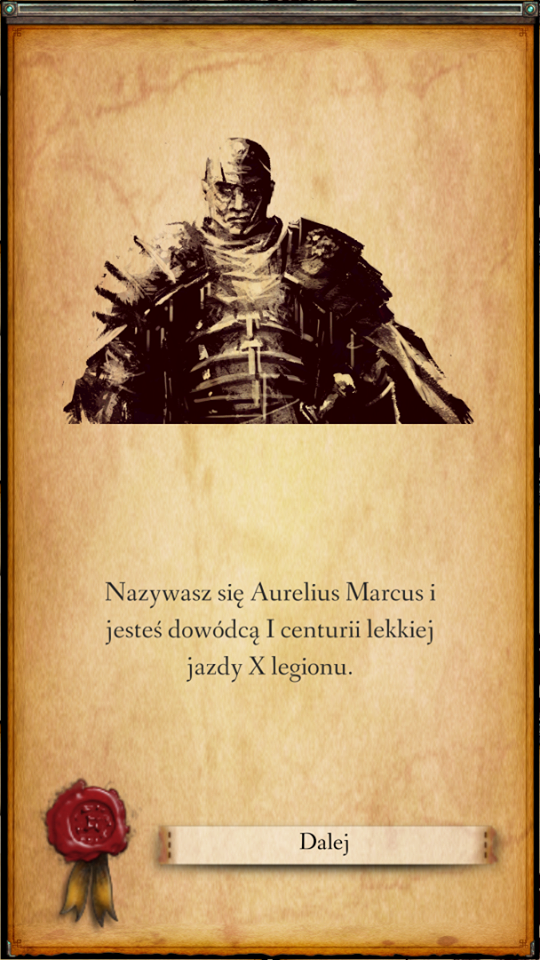
\includegraphics[height=3.0cm,width=1.75cm]{games/rpg_module2.png} 
		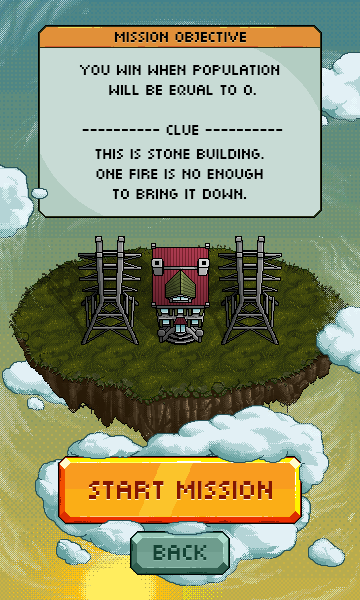
\includegraphics[height=3.0cm,width=1.75cm]{games/fog.png} 
		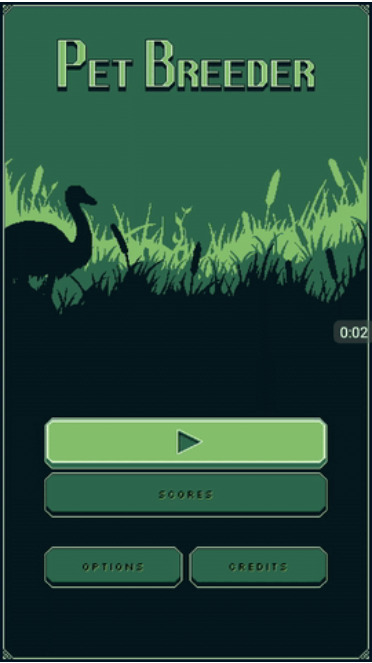
\includegraphics[height=3.0cm,width=1.75cm]{games/pet-breeder.png}
	\item[]
		My games: RPG Module, Finger of God, Pet Breeder.

\end{itemize} 


%\vspace{3cm}
%.



\end{multicols}


%Some of my game jam entries (all are listed on my portfolio {\href{http://www.bobnis.eu}{http://www.bobnis.eu}}):
%\begin{table}[htbp]
%    \centering
%    \begin{tblr}{colspec={X X X X X X }, row{1} = {c}}
%		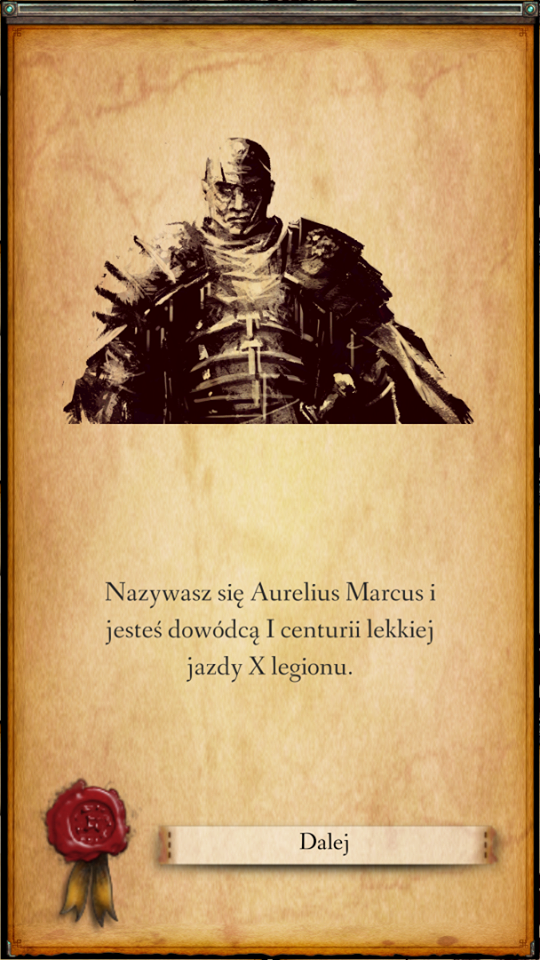
\includegraphics[height=3.0cm,width=1.75cm]{games/rpg_module2.png}
%		&  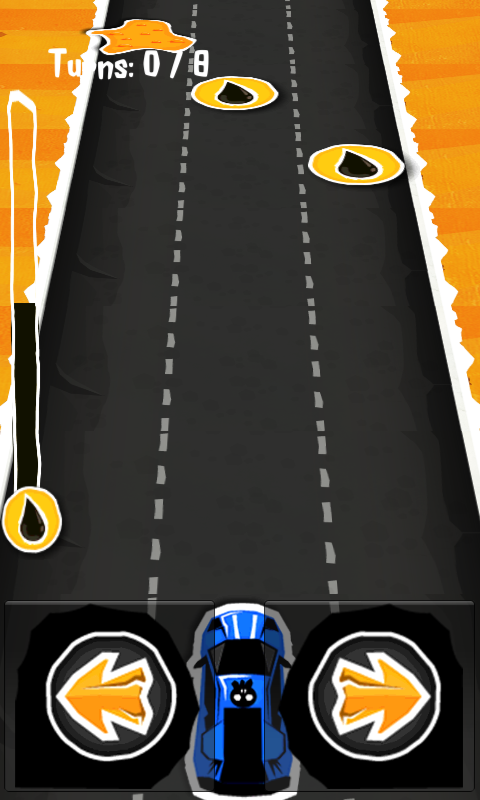
\includegraphics[height=3.0cm,width=1.75cm]{games/zcs.png}
%		& 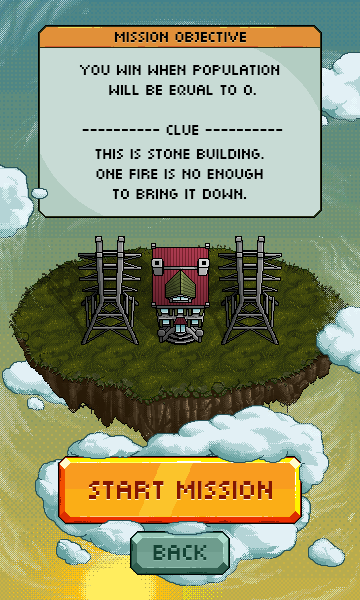
\includegraphics[height=3.0cm,width=1.75cm]{games/fog.png}
%		& 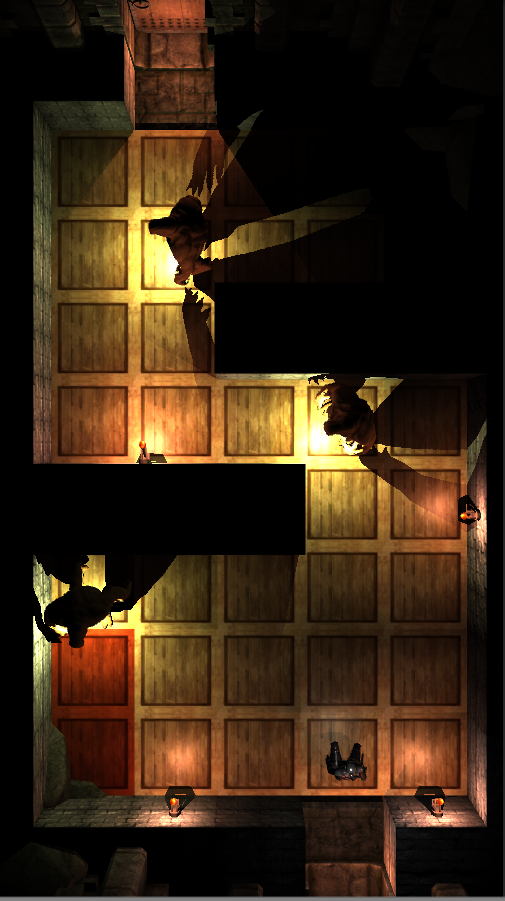
\includegraphics[height=3.0cm,width=1.75cm]{games/stealthRpg.png} 
%		& 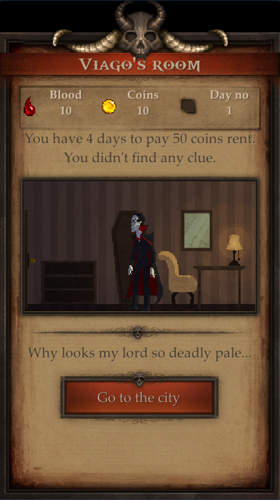
\includegraphics[height=3.0cm,width=1.75cm]{games/viago1.png} 
%		&  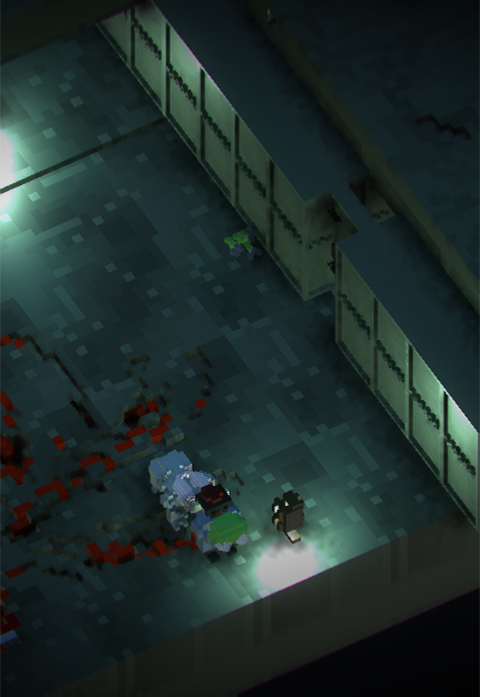
\includegraphics[height=3.0cm,width=1.75cm]{games/scp.png} \\
%
%		  \centering RPG Module
%		& \centering Zombie car smasher
%		& \centering Finger of God
%		& \centering Stealth RPG
%		& \centering Viago the Vampire
%		& \centering SCP-35
%    \end{tblr}
%\end{table}


\end{document}
